\documentclass[a4paper,12pt,fontset=fandol]{ctexart}

\usepackage[a4paper,left=2.5cm,right=2.5cm,top=2.5cm,bottom=2.5cm]{geometry}
\usepackage{graphicx}
\usepackage{subcaption}
\usepackage{booktabs}
\usepackage{longtable}
\usepackage{array}
\usepackage{multirow}
\usepackage{float}
\usepackage{hyperref}
\usepackage{xcolor}
\usepackage{enumitem}
\usepackage{titlesec}
\usepackage{fancyhdr}
\usepackage{setspace}
\usepackage{listings}

\onehalfspacing
\setlength{\headheight}{15pt}
\pagestyle{fancy}
\fancyhf{}
\lhead{生物学数据库及实验大作业实验报告}
\rhead{转座元件知识图谱与智能问答系统}
\cfoot{\thepage}

\titleformat{\section}{\large\bfseries}{\thesection}{0.8em}{}
\titleformat{\subsection}{\normalsize\bfseries}{\thesubsection}{0.8em}{}

\hypersetup{
  colorlinks=true,
  linkcolor=black,
  urlcolor=blue
}

\lstset{
  basicstyle=\ttfamily\small,
  breaklines=true,
  frame=single,
  numbers=left,
  numberstyle=\tiny,
  showstringspaces=false
}

\newcommand{\placeholder}[1]{
  \noindent\colorbox{gray!15}{\parbox{\dimexpr\linewidth-2\fboxsep}{
  \textbf{待补充：} #1}}
}

\newcommand{\figplaceholder}[2]{
  \begin{figure}[H]
    \centering
    \fbox{\rule{0pt}{5cm}\rule{0.85\linewidth}{0pt}}
    \caption{#1}
    \label{#2}
  \end{figure}
}

\title{\textbf{\Huge 生物学数据库及实验大作业实验报告}\\[0.8em]
\Large 转座元件（TE）知识图谱与智能问答系统构建}
\author{}
\date{}

\begin{document}

\maketitle
\thispagestyle{fancy}

\section*{基本信息}
\begin{table}[H]
  \centering
  \renewcommand{\arraystretch}{1.5}
  \begin{tabular}{>{\bfseries}p{3cm} p{11cm}}
    \toprule
    课程名称 & 生物学数据库及实验 \\
    项目题目 & 转座元件（TE）知识图谱与智能问答系统构建 \\
    小组成员 & 蒋贤迪 3240105782 ； 方怡惜 3230106297 \\
    仓库地址 & https://github.com/fff01/TE-.git \\
    开发环境 & Windows + WampServer + PHP + Neo4j + Python \\
    大模型接口 & 阿里云 DashScope / qwen3.5-plus \\
    \bottomrule
  \end{tabular}
\end{table}


\section{项目概述}

本项目围绕“转座元件（TE）知识图谱与智能问答系统构建”展开，目标是从公开文献中抽取与转座元件相关的结构化知识，并将其组织为可检索、可视化和可问答的知识图谱系统。项目以 LINE-1 相关文献为切入点，通过文献抓取、信息抽取、图数据库建模、前端可视化和大模型问答五个环节，完成从原始摘要文本到交互式知识系统的完整流程。

系统面向的主要用户包括课程教师、同学以及希望快速浏览转座元件相关知识的初学者。相较于传统的关键词检索方式，本项目希望通过图谱化结构展示实体之间的关系，并结合自然语言问答接口，提高用户获取 TE 相关知识的效率。

\subsection{研究背景}

转座元件（Transposable Elements, TEs）是基因组中能够发生位置转移的 DNA 序列，在基因组进化、基因表达调控和多种疾病发生过程中具有重要作用。近年来，与 LINE-1、Alu、LTR 等转座元件相关的研究文献持续增长，但这些知识分散在大量论文摘要和研究报告中，普通的文献检索方式难以快速提炼出结构化关系。

知识图谱能够将“实体—关系—实体”的信息组织为图结构，使转座元件、疾病、生物学功能和文献之间的联系更加直观。若再结合大模型的自然语言理解和生成能力，便可以在本地知识库基础上提供更友好的问答入口。因此，本项目将 TE 文献挖掘、图数据库和 RAG 问答三者结合，形成一个面向课程作业的综合型生物信息学系统。

\subsection{系统总体流程}

本项目的整体流程可以概括为五个阶段。首先，从 PubMed 等公共文献数据库中抓取与 LINE-1 等转座元件相关的文献摘要及元数据。其次，利用规则方法和大模型辅助抽取摘要中的 TE、Disease、Function、Paper 等实体及其关系，并输出为结构化结果。随后，对抽取结果进行去重、别名统一和规范化处理，再导入 Neo4j 图数据库，构建知识图谱主存储层。

在数据层完成后，系统通过前端页面将知识图谱局部子图可视化展示出来，支持节点搜索、关系查看和中英文展示切换。最后，用户可以通过网页中的问答界面输入自然语言问题，后端结合 Neo4j 图数据库检索结果与大模型生成能力，返回带有参考文献的学术化答案。整个系统形成了“文献获取 $\rightarrow$ 信息抽取 $\rightarrow$ 图数据库构建 $\rightarrow$ 可视化展示 $\rightarrow$ 智能问答”的闭环。

\figplaceholder{系统总体流程图（建议后续替换为正式架构图）}{fig:overall}


\section{文献挖掘与信息抽取模块}
\subsection{数据来源与抓取策略}
\placeholder{说明使用 PubMed、关键词设计、抓取字段（PMID、Title、Abstract 等）、脚本文件名。}

\subsection{实体识别与关系抽取策略}
\placeholder{说明抽取的实体类型（TE、Disease、Function、Trait、Paper）和关系类型，说明使用的规则、Prompt 或模型。}

\subsection{数据清洗与规范化}
\placeholder{说明去重、别名统一、LINE-1 亚家族关系补充、JSONL/CSV 到图数据库导入前的处理。}

\subsection{文本挖掘策略与准确率评估（简述）}
\placeholder{这是 PDF 明确要求的内容。建议写人工抽样评估：抽样多少篇摘要、看实体抽取是否正确、关系抽取是否合理。}

\begin{table}[H]
  \centering
  \caption{人工抽样准确率评估模板}
  \begin{tabular}{p{3cm} p{3cm} p{3cm} p{4cm}}
    \toprule
    评估对象 & 样本量 & 正确数 & 备注 \\
    \midrule
    实体识别 & \placeholder{例如 50} & \placeholder{例如 43} & \placeholder{说明判断标准} \\
    关系抽取 & \placeholder{例如 30} & \placeholder{例如 24} & \placeholder{说明判断标准} \\
    \bottomrule
  \end{tabular}
\end{table}


\section{图数据库搭建模块}

\subsection{图数据库选型}

本项目选择 Neo4j 作为核心图数据库，而不是仅使用传统关系型数据库。原因在于，本项目的核心数据并不是简单的二维表记录，而是由大量实体及其关系共同构成的知识网络。例如，转座元件与疾病之间存在关联关系，转座元件与生物学功能之间存在调控或参与关系，文献节点又为这些关系提供证据来源；此外，LINE-1 及其亚家族之间还存在层级关系。这些信息天然适合用图结构表示。

若仅采用 MySQL 等关系型数据库，则需要设计多张实体表和关系表，并在查询时大量使用 JOIN 操作。对于“某个转座元件与哪些疾病相关”“哪些文献支持 LINE-1 与某疾病的关联”“L1HS 与 LINE-1 之间是什么关系”这类问题，图数据库能够以更直观的路径形式组织数据，并支持更自然的模式匹配查询。因此，本项目采用 Neo4j 作为知识图谱主存储，将关系型数据库仅保留为可选的辅助组件，而不作为主要知识存储层。

\subsection{Schema 设计}

根据项目需求，我们将知识图谱中的核心对象抽象为四类主要节点：转座元件节点、疾病节点、生物学功能节点和文献节点。所有节点均以名称或主键属性作为识别依据，以支持去重、归一化和后续检索。

\subsubsection*{节点标签设计}

\begin{table}[H]
  \centering
  \caption{节点设计}
  \begin{tabular}{p{2.5cm} p{5cm} p{6cm}}
    \toprule
    节点类型 & 主要属性 & 说明 \\
    \midrule
    TE & name, category, description, source\_group & 表示转座元件及其亚家族，例如 LINE-1、L1HS、Alu 等 \\
    Disease & name, source\_group & 表示疾病实体，例如阿尔茨海默病、乳腺癌等 \\
    Function & name, source\_group & 表示生物学过程或功能实体，例如逆转录转座、DNA damage 等 \\
    Paper & name, pmid, source\_group & 表示文献证据节点，通常以论文标题和 PMID 标识 \\
    \bottomrule
  \end{tabular}
\end{table}

在实际实现中，节点导入采用 ``名称唯一'' 的策略。对于 TE、Disease、Function 三类实体，均以 `name` 作为主要去重键；对于 Paper 节点，优先保留 PMID 与标题信息，以便后续在问答模块和可视化模块中进行证据溯源。

\subsubsection*{关系类型设计}

\begin{table}[H]
  \centering
  \caption{关系设计}
  \begin{tabular}{p{3cm} p{4cm} p{6cm}}
    \toprule
    关系类型 & 示例 & 说明 \\
    \midrule
    SUBFAMILY\_OF & L1HS $\rightarrow$ LINE-1 & 表示亚家族与总家族之间的层级关系 \\
    BIO\_RELATION & LINE-1 $\rightarrow$ 阿尔茨海默病 & 表示转座元件与疾病或功能之间的生物学关联，具体谓词写入关系属性 \\
    EVIDENCE\_RELATION & Paper $\rightarrow$ TE/Disease/Function & 表示文献对实体或知识项的支持关系 \\
    \bottomrule
  \end{tabular}
\end{table}

其中，\texttt{SUBFAMILY\_OF} 是本项目中非常重要的一类结构化关系。队友提供了 LINE-1 谱系中的多个亚家族信息，因此系统在知识图谱中专门补充了 \texttt{L1HS}、\texttt{L1PA2}、\texttt{L1PB1}、\texttt{L1MA1} 等节点，并通过 \texttt{SUBFAMILY\_OF} 将其统一连接到 \texttt{LINE-1}。这一设计使知识图谱不仅能表达功能和疾病关系，还能表达转座元件内部的谱系结构。

\texttt{BIO\_RELATION} 用于统一存储 TE 与 Disease、Function 之间的生物学关系。考虑到原始文献抽取结果中的关系词较多，若直接将所有谓词都建成独立的边类型，会造成边类型碎片化，不利于后续查询和维护。因此，系统将这类边统一表示为 \texttt{BIO\_RELATION}，而将具体谓词写入关系属性 \texttt{predicate}，同时保留 PMID 集合作为证据引用。

\texttt{EVIDENCE\_RELATION} 则用于文献溯源。它连接文献节点与 TE、Disease、Function 等实体节点，使系统在回答问题时不仅能给出结论，还能返回来源文献。

\subsubsection*{关系属性设计}

本项目中较重要的关系属性包括：

\begin{itemize}[leftmargin=2em]
  \item \texttt{predicate}：表示具体生物学关系词，如“促进”“相关”“导致”“参与”等；
  \item \texttt{pmids}：记录支持该关系或实体的 PMID 列表；
  \item \texttt{copies}：用于 \texttt{SUBFAMILY\_OF} 关系中，记录亚家族拷贝数；
  \item \texttt{source}：用于标记关系来源，如谱系参考或抽取结果。
\end{itemize}

这种设计兼顾了结构统一性和语义细节。在图数据库中，边类型保持简洁，而具体语义和证据保存在关系属性中，有利于问答模块进行检索增强生成。

\subsection{数据导入与查询}

本项目的数据导入主要分为四步：

\begin{enumerate}[leftmargin=2em]
  \item 导入 TE、Disease、Function、Paper 四类节点；
  \item 导入 LINE-1 与其亚家族之间的 \texttt{SUBFAMILY\_OF} 关系；
  \item 导入 TE 与 Disease、Function 之间的 \texttt{BIO\_RELATION}；
  \item 导入 Paper 与实体之间的 \texttt{EVIDENCE\_RELATION}，用于证据溯源。
\end{enumerate}

在实现层面，系统首先通过 Python 脚本对原始抽取结果进行去重与规范化，例如统一 `LINE-1 / LINE1 / L1` 的写法，并补充亚家族层级关系。清洗后的数据再被转换为 Cypher 导入脚本，批量导入 Neo4j。为了避免重复插入节点或关系，导入时统一使用 `MERGE` 而非简单 `CREATE`。

当前项目中与图数据库相关的关键脚本和导入文件包括：

\begin{itemize}[leftmargin=2em]
  \item \texttt{normalize\_line1\_graph.py}：对抽取结果做去重与规范化；
  \item \texttt{import\_graph\_node\_names.cypher}：导入节点；
  \item \texttt{import\_line1\_subfamilies.cypher}：导入 LINE-1 亚家族层级关系；
  \item \texttt{import\_core\_relations.cypher}：导入 TE 与 Disease/Function 的核心关系；
  \item \texttt{import\_paper\_relations.cypher}：导入文献证据关系。
\end{itemize}

在查询层面，Neo4j 使用 Cypher 语言进行图模式匹配。例如：

\begin{itemize}[leftmargin=2em]
  \item 查询某个 TE 的亚家族：
  \texttt{MATCH (a:TE)-[:SUBFAMILY\_OF]->(b:TE \{name:'LINE-1'\}) RETURN a,b}
  \item 查询某个 TE 相关的疾病：
  \texttt{MATCH (a:TE)-[r:BIO\_RELATION]->(b:Disease) RETURN a,r,b}
  \item 查询支持某一关系的文献证据：
  \texttt{MATCH (p:Paper)-[r:EVIDENCE\_RELATION]->(t:TE) RETURN p,r,t}
\end{itemize}

这一图数据库设计为后续两个模块提供了直接支撑：前端可视化模块通过图谱节点和边进行展示，智能问答模块则通过 Cypher 检索相关子图路径，并将检索到的结构化知识作为大模型生成回答的上下文。

\section{知识图谱可视化展示模块}

\subsection{前端展示设计}

本项目构建了一个面向课程演示和知识浏览的图谱前端页面。页面整体采用左右分栏结构：左侧为知识图谱展示区域，右侧为智能问答区域。用户可以在左侧浏览转座元件相关的局部知识网络，在右侧直接输入自然语言问题并查看回答结果。该设计能够将“图谱展示”和“智能问答”两个模块整合在同一页面中，便于演示和交互。

在数据组织上，图谱页面当前主要围绕 LINE-1 及其相关实体展开，包括：

\begin{itemize}[leftmargin=2em]
  \item TE 节点：例如 LINE-1、L1HS、Alu 等；
  \item Disease 节点：例如阿尔茨海默病、乳腺癌等；
  \item Function 节点：例如逆转录转座、DNA damage 等；
  \item Paper 节点：用于表示支持性文献；
  \item 层级关系边与证据关系边。
\end{itemize}

为了兼顾展示效果和课程答辩使用场景，前端还加入了中英文展示切换。系统在展示层对部分疾病、功能和关系名称做了中英文映射，但底层数据库仍保留较规范的原始命名，以保证检索一致性。

\subsection{核心交互功能}

当前图谱展示模块实现了以下核心交互功能：

\begin{itemize}[leftmargin=2em]
  \item \textbf{节点搜索与定位}：用户可以通过搜索快速定位某个转座元件、疾病或功能节点；
  \item \textbf{节点点击详情}：点击节点后，可在详情区域查看实体类型和关联信息；
  \item \textbf{关系点击查看证据}：点击边后，可查看关系类型及其相关证据描述；
  \item \textbf{图谱布局重排}：页面支持重新布局，使节点在初始展示时尽量分散，减少重叠；
  \item \textbf{局部高亮}：点击节点或边后，可以重点突出局部子图，减轻全图过密导致的阅读困难；
  \item \textbf{中英文切换}：支持面向中文展示和英文展示两种模式。
\end{itemize}

在可视化实现中，项目对布局参数进行了多轮调节，以尽量降低节点和标签重叠问题。特别是对文献节点和证据关系进行了较强的排斥与长度控制，从而让核心 TE、Disease、Function 节点在初始视图中更清晰。

\subsection{图谱页面与后端模块的关系}

该可视化模块并不是孤立页面，而是和图数据库及智能问答系统直接联动：

\begin{itemize}[leftmargin=2em]
  \item 图谱展示使用的是从 Neo4j 组织导出的本地子图数据；
  \item 节点和边的展示逻辑与 Neo4j 中的标签和关系设计保持一致；
  \item 右侧问答面板通过 PHP 后端访问 Neo4j，并将问答结果与图谱页面整合；
  \item 文献节点与关系证据共同支持“可视化展示 + 问答溯源”的完整流程。
\end{itemize}

因此，该模块在整个系统中起到桥梁作用：它既是知识图谱的图形化界面，也是智能问答系统的人机交互入口。

\subsection{网站主要功能截图}

\placeholder{这是 PDF 明确要求的内容。建议至少准备 4 张：图谱首页、节点详情、问答结果、Neo4j 查询结果。}
\begin{figure}[H]
  \centering
  \begin{subfigure}[t]{0.48\linewidth}
    \centering
    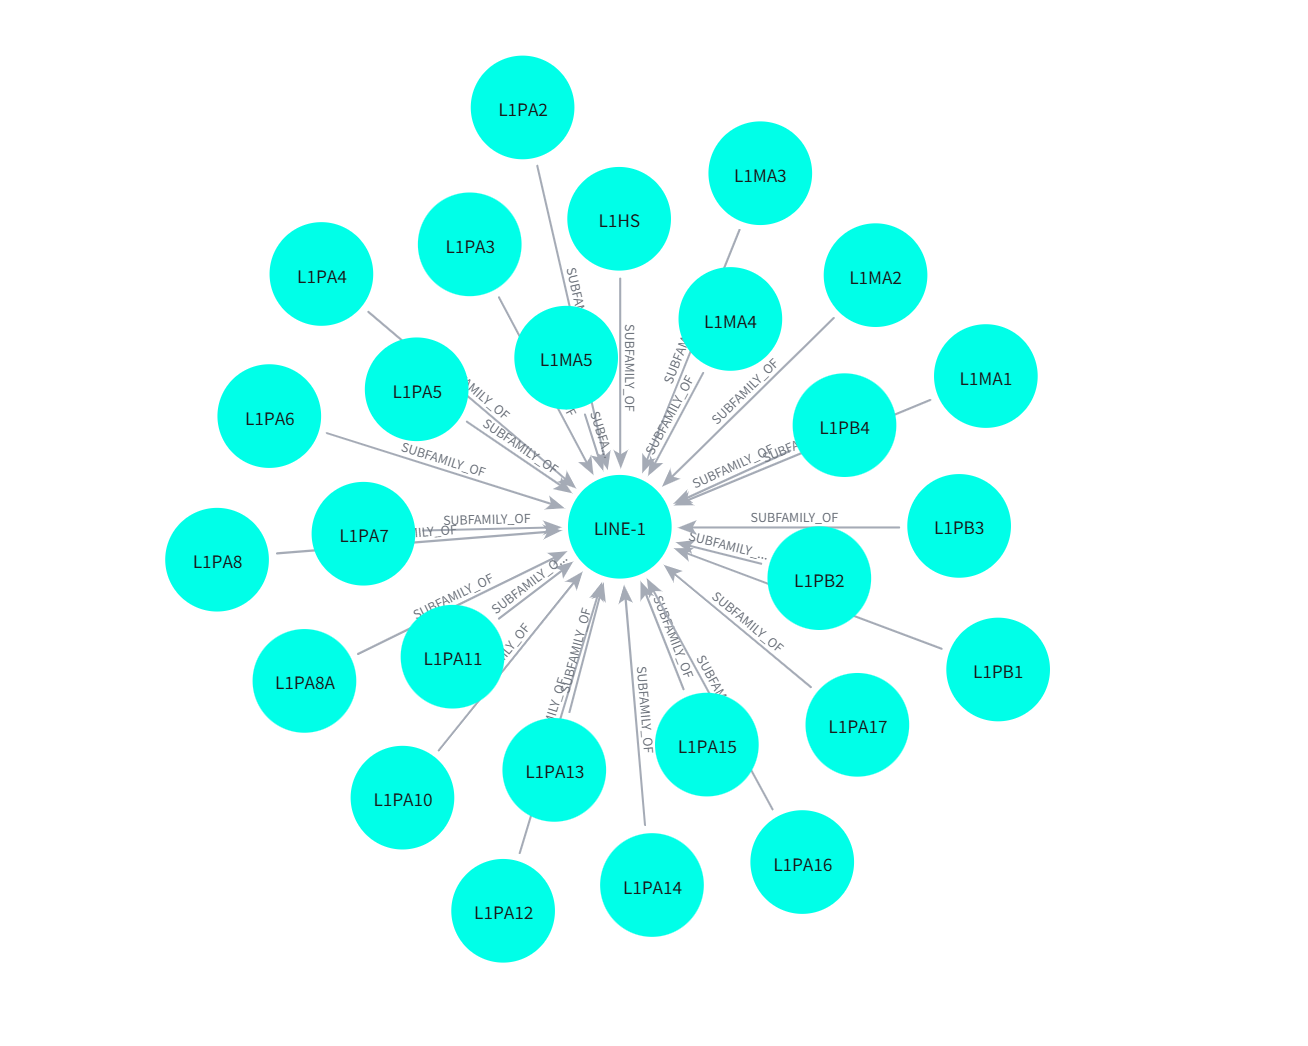
\includegraphics[width=\linewidth]{figures/fig_neo4j_query.png}
    \caption{Neo4j Query 中的 LINE-1 亚家族谱系结果}
    \label{fig:neo4j-query}
  \end{subfigure}
  \hfill
  \begin{subfigure}[t]{0.48\linewidth}
    \centering
    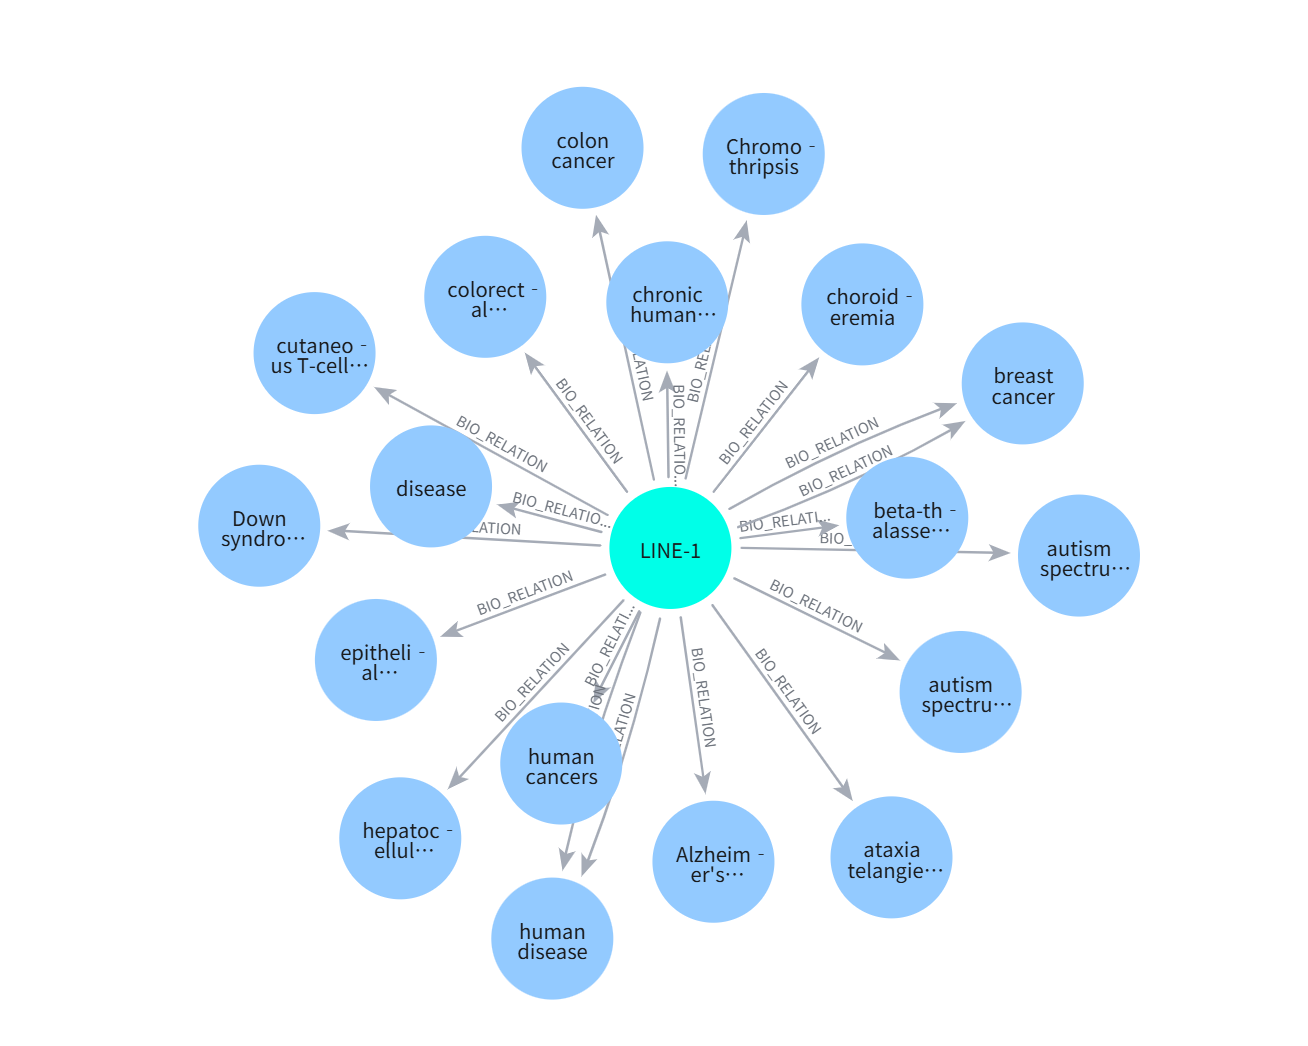
\includegraphics[width=\linewidth]{figures/fig_neo4j_visualisation.png}
    \caption{Neo4j 可视化视图中的局部图谱结构}
    \label{fig:neo4j-visualisation}
  \end{subfigure}
  \caption{图数据库查询结果与可视化展示}
  \label{fig:web-neo4j-pair}
\end{figure}

\figplaceholder{图谱主页截图占位}{fig:web-home}
\figplaceholder{节点详情或关系详情截图占位}{fig:web-detail}
\figplaceholder{问答系统截图占位}{fig:web-qa}

\section{基于大模型的智能问答系统}

\subsection{系统目标}

本项目在网站中集成了一个基于本地知识库的智能问答模块。用户可以直接输入自然语言问题，例如“LINE-1 相关疾病有哪些”“LINE-1 相关功能是什么”“L1HS 和 LINE-1 是什么关系”或“哪些文献支持 LINE-1 与阿尔茨海默病相关”。系统需要结合本地 Neo4j 图数据库中的知识，给出结构化且带有参考文献的回答，而不是脱离知识库进行自由生成。

与普通聊天系统不同，本项目的问答模块强调“基于本地知识库回答”和“附带证据来源”两点。一方面，系统回答的核心内容应来自已导入的转座元件知识图谱；另一方面，回答中需要尽可能返回 PMID 或文献标题，以满足课程项目对于知识溯源的要求。

\subsection{RAG 架构设计}

本系统的智能问答模块采用检索增强生成（Retrieval-Augmented Generation, RAG）架构。其核心思想是：先从本地图数据库中检索与用户问题相关的结构化知识，再将这些检索结果作为上下文提供给大模型，由模型生成通顺、客观、学术化的自然语言回答。

考虑到完全自由的 Text2Cypher 在课程项目场景下容易产生不可控的错误，本项目采用了“模板优先、Text2Cypher 兜底”的策略。对于常见且结构清晰的问题，优先匹配模板化查询；仅在模板未命中时，才进入受限的 Text2Cypher 生成流程。这种设计在保持灵活性的同时，提高了系统稳定性和可演示性。

\begin{figure}[H]
  \centering
  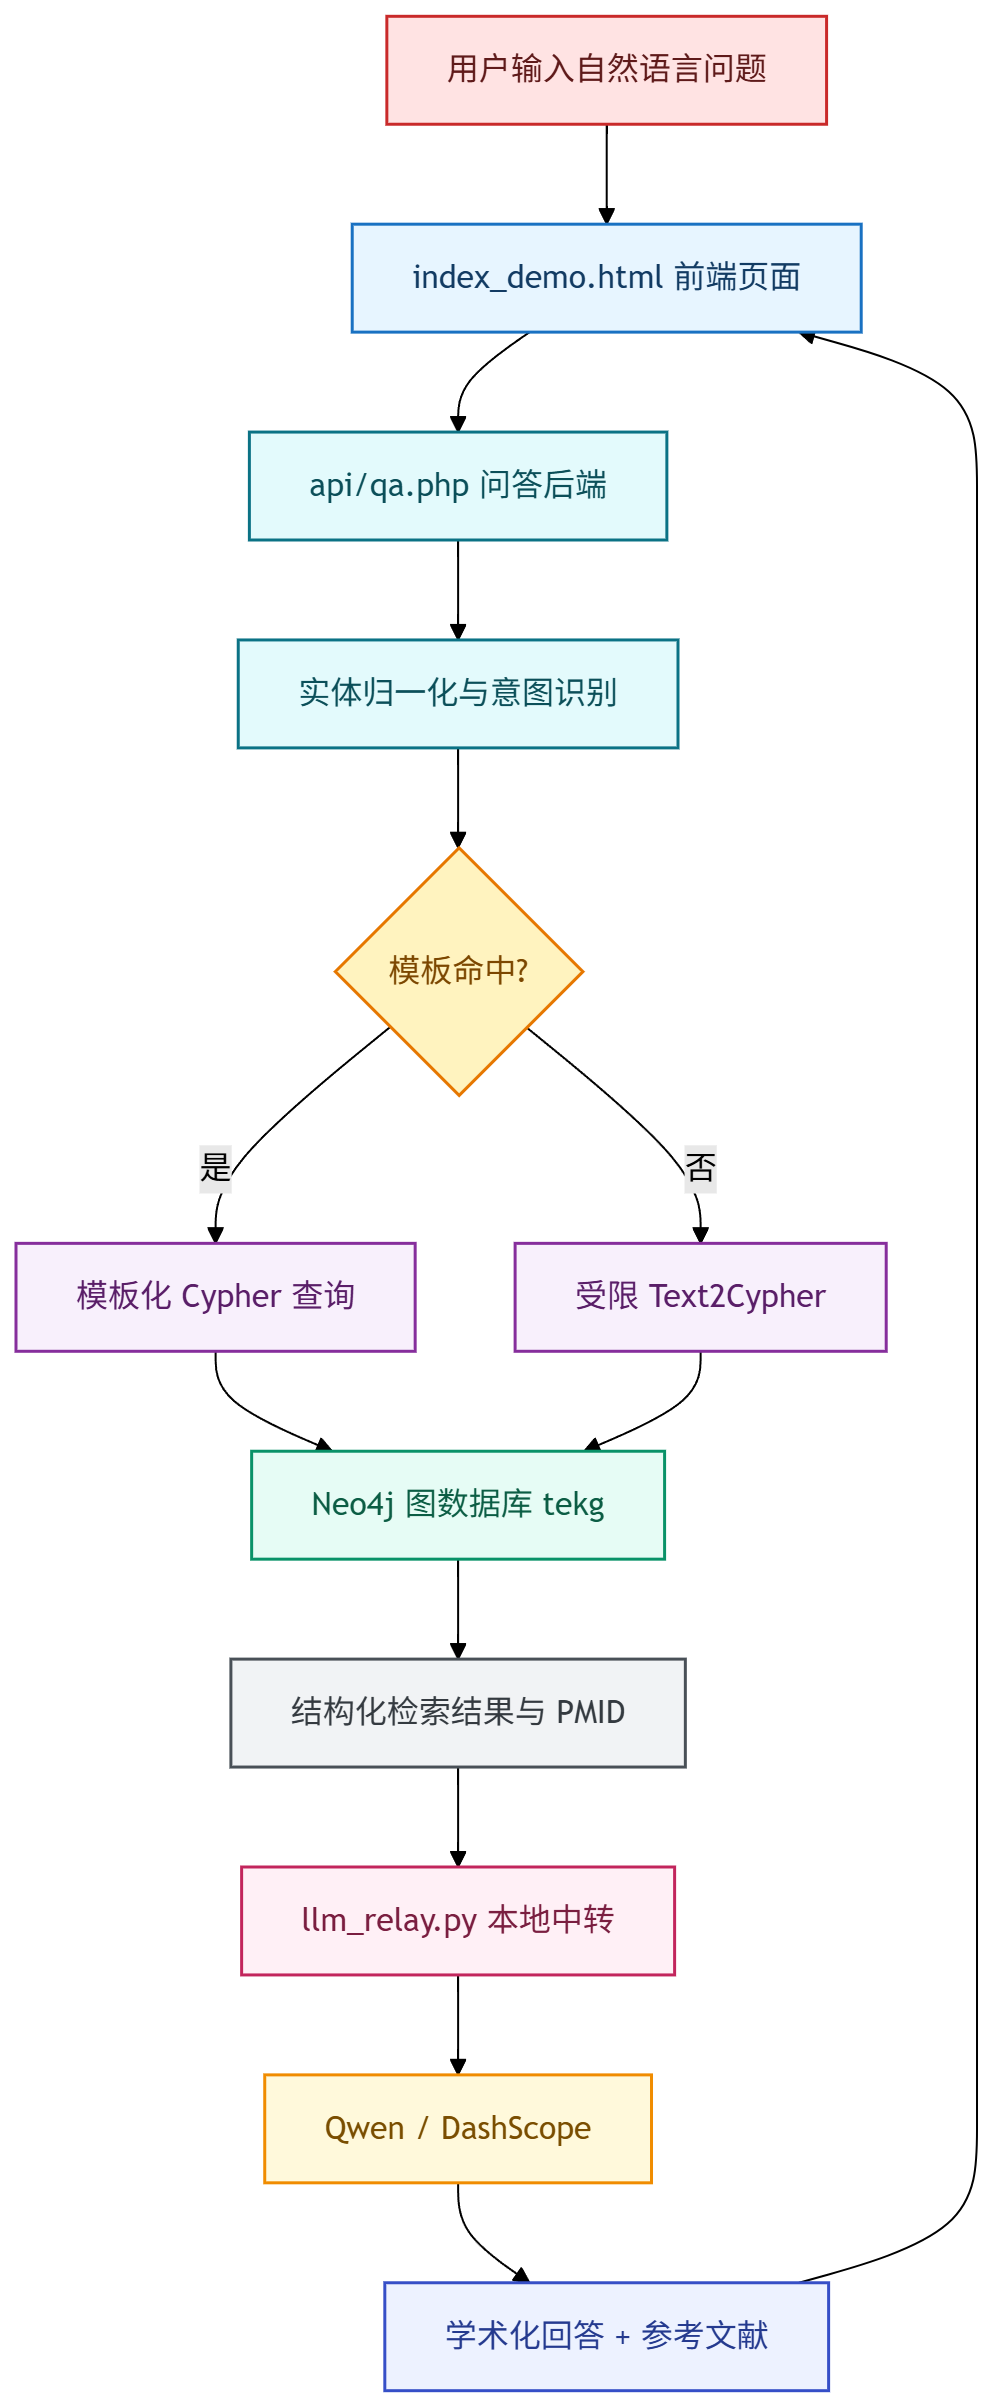
\includegraphics[width=0.88\linewidth]{figures/fig_rag_architecture.png}
  \caption{基于 Neo4j 检索与 Qwen 生成的 RAG 问答架构}
  \label{fig:rag}
\end{figure}

\subsection{Prompt 设计思路}

Prompt 设计的核心目标是约束模型只基于本地检索结果作答，并以较为严谨的学术语言组织回答。具体而言，本项目在提示词设计中遵循以下原则：

\begin{itemize}[leftmargin=2em]
  \item 明确要求模型优先依据 Neo4j 检索结果回答，而不是自由发挥；
  \item 要求回答采用固定结构，如“结论”“关键点”“参考文献”三段式；
  \item 要求在可提供文献时尽量附带 PMID 或文献标题；
  \item 若知识库中缺乏充分证据，则明确说明“本地知识库暂无充分证据”，避免模型编造关系；
  \item 对输出语言进行约束，使其尽量保持客观、严谨和适合作业展示的风格。
\end{itemize}

此外，系统还对一些常见术语进行了后处理规范化，例如疾病名称中英混杂、实体名称别名不统一等问题，以提升最终回答的可读性和一致性。

\subsection{问答流程实现}

本项目中问答模块的实际处理流程如下：

\begin{enumerate}[leftmargin=2em]
  \item 用户在前端页面输入自然语言问题；
  \item 前端将问题发送到 PHP 后端接口 \texttt{api/qa.php}；
  \item 后端首先进行实体归一化与意图识别，例如识别问题是否属于“相关疾病”“相关功能”“文献证据”“亚家族关系”等类型；
  \item 若问题命中模板，则直接生成模板化 Cypher 查询；若未命中，则进入受限 Text2Cypher 路径；
  \item 在 Neo4j 图数据库中执行查询，得到相关节点、关系和 PMID；
  \item 将结构化检索结果整理为上下文；
  \item 后端通过本地中转服务 \texttt{llm\_relay.py} 调用 Qwen 模型；
  \item 大模型基于检索上下文生成自然语言回答，并返回给前端；
  \item 前端将回答以 Markdown 形式渲染，同时保留回退机制：若模型调用失败，则至少给出基于本地检索结果生成的结构化答案。
\end{enumerate}

这种设计保证了系统在两种情况下都能工作：在理想网络条件下，系统可输出较完整的大模型增强回答；在模型接口不可用时，系统仍能依赖本地图数据库返回基础结构化答案，避免整页功能失效。

\subsection{当前支持的问题类型}

结合当前系统实现，问答模块已经支持以下几类典型问题：

\begin{itemize}[leftmargin=2em]
  \item 某个转座元件相关的疾病，例如“LINE-1 相关疾病”；
  \item 某个转座元件相关的功能，例如“LINE-1 相关功能”；
  \item 某个亚家族与总家族的关系，例如“L1HS 和 LINE-1 是什么关系”；
  \item 某个实体-疾病对的证据查询，例如“哪些文献支持 LINE-1 与阿尔茨海默病相关”；
  \item 某个实体的文献证据查询，例如“L1HS 有哪些文献证据”。
\end{itemize}

这些问题类型已经覆盖了课程项目答辩中最适合演示的一批典型用例。

\subsection{问答示例}

\begin{figure}[H]
  \centering
  \begin{subfigure}[t]{0.48\linewidth}
    \centering
    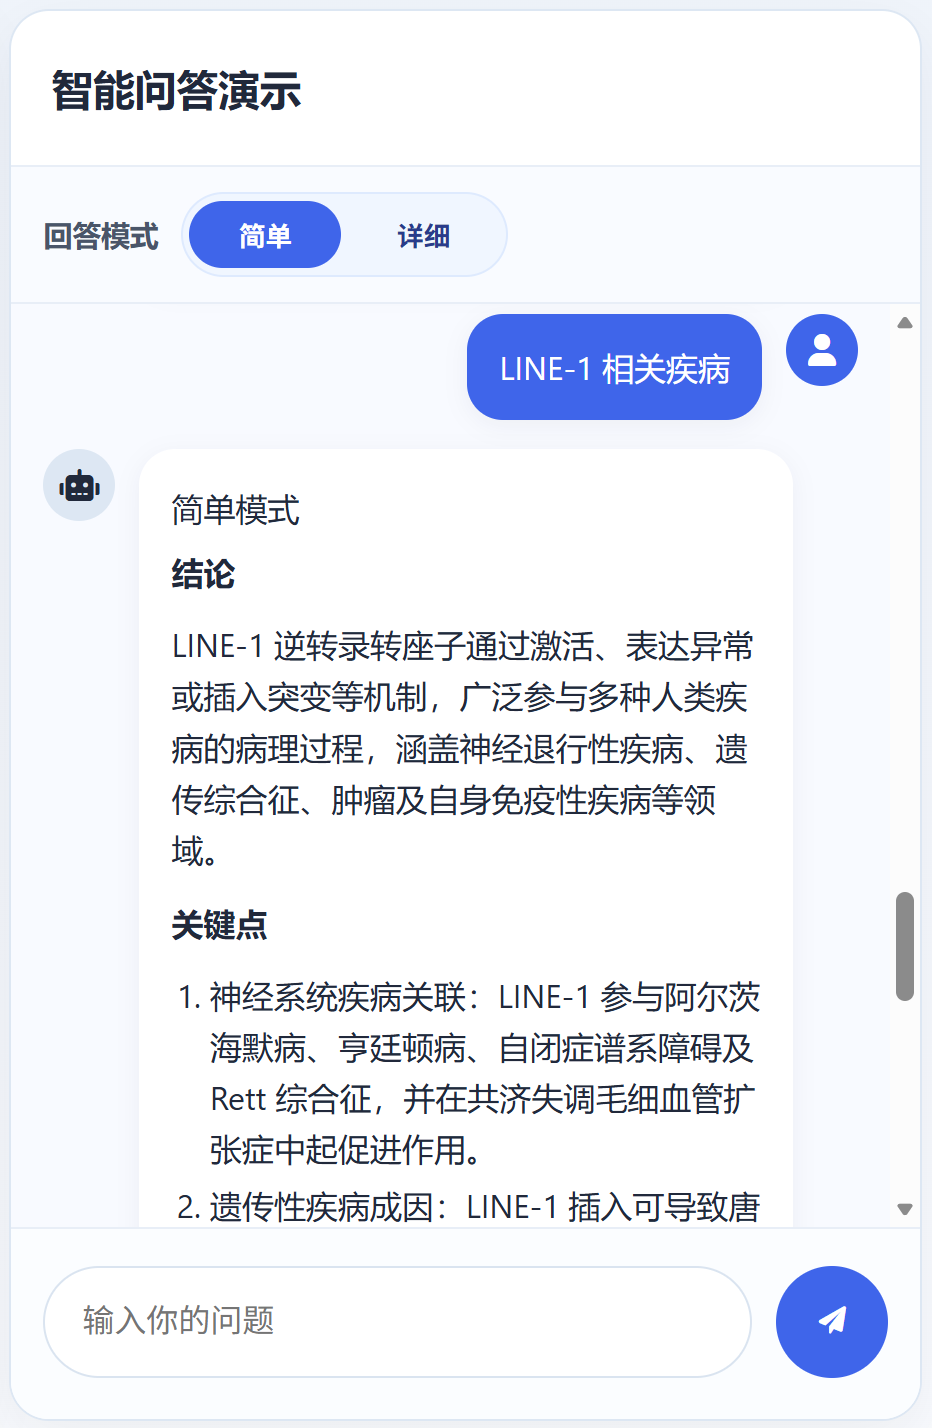
\includegraphics[width=\linewidth]{figures/fig_qa_simple.png}
    \caption{简单模式问答示例}
    \label{fig:qa-simple}
  \end{subfigure}
  \hfill
  \begin{subfigure}[t]{0.48\linewidth}
    \centering
    
\includegraphics[width=\linewidth]{figures/fig_qa_detailed.png}
    \caption{详细模式问答示例}
    \label{fig:qa-detailed}
  \end{subfigure}
  \caption{智能问答模块的简单模式与详细模式展示}
  \label{fig:qa-mode-pair}
\end{figure}

\section{系统实现与关键文件说明}

为方便说明项目整体结构，本项目将主要代码分为文献抓取与信息抽取、图数据库导入、前端可视化展示以及智能问答后端四个部分。各关键文件作用如下表所示。

\begin{longtable}{p{4cm} p{9cm}}
  \toprule
  文件/模块 & 说明 \\
  \midrule
  index\_demo.html & 图谱展示与问答前端页面 \\
  api/qa.php & 智能问答后端接口 \\
  llm\_relay.py & 本地大模型中转服务 \\
  normalize\_line1\_graph.py & 数据清洗与命名规范化脚本 \\
  import\_*.cypher & Neo4j 节点与关系导入脚本 \\
  output.jsonl / normalized\_output.jsonl & 文献信息抽取结果与规范化结果 \\
  \bottomrule
\end{longtable}

\section{小组成员分工}

\begin{table}[H]
  \centering
  \caption{小组成员分工}
  \renewcommand{\arraystretch}{1.35}
  \begin{tabular}{p{2.3cm} p{10.5cm}}
    \toprule
    成员 & 主要贡献 \\
    \midrule
    \multirow{4}{*}{甲}
      & 负责 PubMed 文献检索与 LINE-1 相关摘要数据整理。 \\
      & 负责摘要级实体与关系的初步抽取，以及原始结构化结果输出。 \\
      & 负责提供文本挖掘模块的关键词设计、抽取样例与评估材料。 \\
      & 参与文献挖掘结果核对，并协助完善实验报告相关内容。 \\
    \midrule
    \multirow{4}{*}{乙}
      & 负责 Neo4j 图数据库建模、节点关系导入与数据规范化处理。 \\
      & 负责知识图谱可视化前端页面开发、双语展示与交互效果调整。 \\
      & 负责基于本地知识库和大模型接口的智能问答模块实现与联调。 \\
      & 负责系统集成测试、演示流程整理及实验报告主体撰写。 \\
    \bottomrule
  \end{tabular}
\end{table}

\section{总结与不足}

目前，本项目已经实现了从文献获取、信息抽取、图数据库建模、图谱可视化展示到基于本地知识库的智能问答的完整闭环。系统能够围绕 LINE-1 及其亚家族构建知识子图，支持疾病、功能和文献证据的图谱化展示，并可通过自然语言问题从本地知识图谱中检索证据，再结合大模型生成带参考文献的回答。

项目当前仍存在若干局限。首先，图谱中的部分实体名称仍存在中英文混杂和粒度不完全统一的问题，后续仍可继续规范化。其次，当前前端以演示型子图为主，若扩展到更大范围的 TE 类型，还需要进一步优化动态加载与布局策略。最后，问答模块虽然已经支持模板化查询和受限的 Text2Cypher 思路，但在更复杂、开放的问题场景下仍有提升空间。

总体而言，本项目已经达到课程大作业的核心目标，并为后续扩展到更大规模的 TE 文献知识图谱提供了可复用的技术框架。

\section*{正式写作前的材料准备清单}
\begin{itemize}[leftmargin=2em]
  \item 文献抓取与信息抽取脚本名称、运行流程与关键词策略
  \item 实体类型与关系类型清单
  \item Neo4j 节点与关系设计表
  \item RAG 架构图
  \item Prompt 设计说明
  \item 3 到 5 张系统截图
  \item 2 到 3 条典型问答示例
  \item 人工抽样准确率评估结果
  \item 小组成员分工说明
  \item GitHub 仓库地址与主要文件说明
\end{itemize}


\end{document}
